\section{Parameter Estimation using Optimization}
In this section two methods for optimization will be investigated. The base of the implementation is in this case a Matlab script which is fed with test data along with the model simulation, whose task is to fit the model output to the test data by adjusting one or more parameters in the model. In this case the model representation supplied to the script is a Simulink model, which can then be run by the script whenever needed and the script can modify the parameters to be adjusted. The process is iterative in most cases.

\subsection{The Optimization Problem}
The basic scheme for the optimization problem is given in \figref{SensToolSchema}.
%
\begin{figure}[H]
	\centering
	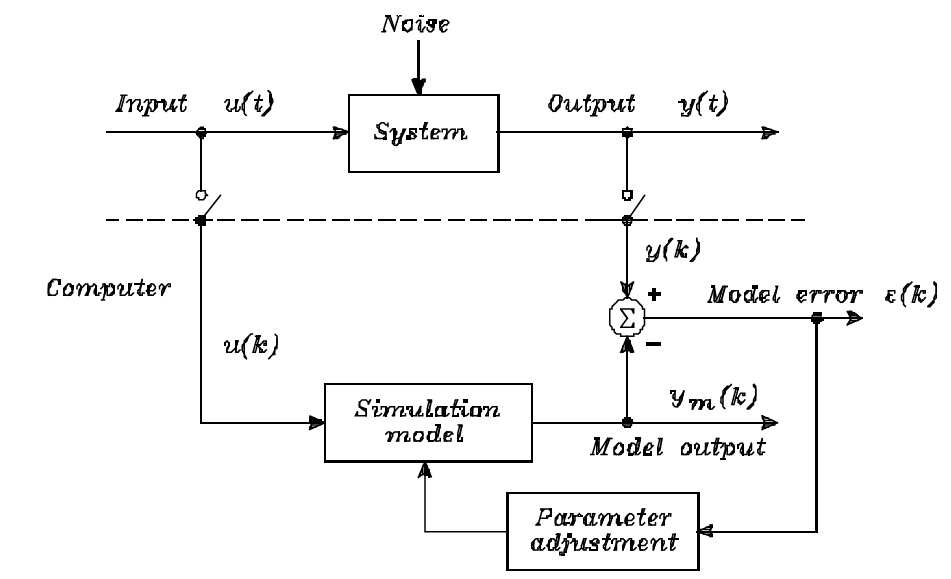
\includegraphics[scale=0.4]{figures/SensToolSchema}
	\caption{Schematic of the optimization problem}
	\label{SensToolSchema}
\end{figure}
%
The provided data is taken from an initial value test of the Cubli hanging down like a pendulum, see \appref{impulseResponseAppendix}.
As the operating angle goes from \si{-0,15\ to\ 0,15\ rad}, the behavior at this range will be better if the fit is done between this operating points. 

Furthermore, the nonlinear model is used to accurately describe the oscillatory behavior of the pendulum. The model is modified such that it describes the system as a regular pendulum without the dynamics of the reaction wheel, in order to match the test conditions under which the data was extracted, as seen in \figref{blockDiagramSenseTool},
%
\begin{figure}[H]
	  \begin{tikzpicture}[ auto,
                       thick,                         %<--setting line style
                       node distance=1.5cm,             %<--setting default node distance
                       scale=0.75,                     %<--|these two scale the whole thing
                       every node/.style={scale=0.62}, %<  |(always change both)
                       >/.tip={Triangle[angle=40:5pt]}
                       ]

    %-- Blocks creation --%
    \draw
      % DIRECT TERM %
      node[shape=coordinate][](input1) at (0,0){}
      node[shape=coordinate][](feedForward) at (0.5,0){}
      node(sum1) at (2.25,0) [sum]{\si{\sum}}
      node(sum2) at (3.75,0) [sum]{\si{\sum}}

      node(torque2rotacc1) at (6.85,0) [block]{\large \si{\frac{1}{J_F + J_w + m_w \cdot {l_w}^{2}}}}

      node(integration1) at (10.75,0) [block] {\large \si{\frac{1}{s}}}
      node(integration2) at (14.2,0) [block] {\large \si{\frac{1}{s}}}

      node[shape=coordinate][](output) at (15.3,0){}
      node[shape=coordinate][](veloFeedbackNode) at (11.8,0){}
      
    ;
    \draw
      % FEEDBACKS %
      node(veloFeedback) at (7,-2) [block] {\large \si{B_F}}
      node(angleFeedback) at (8,-4) [block] {\large \si{(m_F \cdot l_F + m_w \cdot l_w)g}}
    ;
    %-- Block linking --%
    % INPUT %
    \draw[-](input1)        -- node{\large \si{\tau_m(s)}}(feedForward);
    \draw[->](feedForward)  -- (sum1);

    % OUTPUT %
    \draw[-](integration2)  -- (output);
    \draw[->](output)       -- node {\large \si{\theta_{F}(s)}} (17,0);

    % DIRECT TERM %
    \draw[->] (sum1)            -- (sum2);
    \draw[->] (sum2)            -- (torque2rotacc1);
    \draw[->] (torque2rotacc1)  -- node{\large \si{\alpha_F(s)}}(integration1);
    \draw[->] (integration1)    -- node{\large \si{\omega_F(s)}}(integration2);

    % FEEDBACKS

    \draw[->] (output)           |- (angleFeedback);
    \draw[->] (angleFeedback)    -| (sum1);

    \draw[->] (veloFeedbackNode) |- (veloFeedback);
    \draw[->] (veloFeedback)     -| (sum2);

    %-- Nodes --%
    \draw%--------------------------------------------------------------
      node at (input1)            [shift={(-0.04, -0.05 )}] {\Large \textopenbullet}
      node at (output)            [shift={( 0.007, -0.05 )}] {\Large \textbullet}
      node at (veloFeedbackNode)  [shift={( 0.007, -0.05 )}] {\Large \textbullet}
    ;

    %-- Summation signs --%
      \draw%--------------------------------------------------------------

      node at (sum1) [right = -6.6mm, below = .6mm] {$-$}
      node at (sum1) [right = -3mm, below = 3.9mm]  {$+$}
      node at (sum2) [right = -6.6mm, below = .6mm] {$+$}
      node at (sum2) [right = -3mm, below = 3.9mm]  {$-$}

    ;

  \end{tikzpicture}
	\centering
	\caption{Block diagram of the system as a regular pendulum with the wheel fixed to the frame.}
	\label{blockDiagramSenseTool}
\end{figure}
%
 In order to minimize the difference between the data points measured in test and the output of the model, a function to describe such a relationship is needed. The performance function used to describe goodness of the fit, is a mean square error function.
%
\begin{flalign}
	\eq{P(\vec{\theta})} {\frac{1}{2N}\sum_{k = 1}^{N} \left(\vec{y}(kT) - \vec{y_m}(kT, \vec{\theta})\right)^2 } &
\label{performanceFunction}
\end{flalign}
%
\hspace{6mm} Where:\\
\begin{tabular}{ p{1cm} l l l}
& \si{\vec{\theta}}   & is the parameter(s) to be adjusted                  & \\
& \si{N}              & is the degrees of freedom for each parameter        & \\
& \si{k}              & is the sample indexes, \si{k=1,\ 2,} ...\si{,\ N}   & \\
& \si{T}              & is the sampling time                                & \\
& \si{\vec{y}}        & is the test measurement output vector               & \\
& \si{\vec{y_m}}      & is the model output vector                          & \\
\end{tabular}

A normal mean square error function is only divided by the degrees of freedom, \si{N}, but in tis case is divided by \si{2N} to cancel out the factor which arises when computing its gradient. This only gives the function a constant offset and does not have any impact when minimizing it.

\subsection{Optimization using the Gradient}
One way of solving the optimization problem is through the use of the gradient. It indicates in which direction the steepest descent (or ascent) is found in an infinitesimal surrounding of a given starting point.

For a function \si{f(\vec{x})} with a change in \si{\vec{x}} of \si{\vec{\delta}}, the following can be obtained from the Taylor series.
%
\begin{flalign}
  f(\vec{x}+\vec{\delta}) &\approx f(\vec{x}) + \vec{g}^T \vec{\delta} + \frac{1}{2} \vec{\delta}^T \vec{H}\vec{\delta} &
\label{taylorApproximation}
\end{flalign}
%
\hspace{6mm} Where:\\
\begin{tabular}{ p{1cm} l l l}
& \si{\vec{g}} 					    	   & is the gradient \si{\nabla f(\vec{x})} & \\
& \si{\vec{H}} 					    	   & is the Hessian                         & \\
& \si{\vec{\delta}} 					   & is the change in \si{\vec{x}}          & \\
\end{tabular}

%Then the change in \si{f(x)} as \si{||\vec{\delta}||_2 \rightarrow 0} can be approximated as follows.
%%
%\begin{flalign}
%  \Delta f(x) &\approx \vec{g}^T \vec{\delta} = ||\vec{g}||_2 \ ||\vec{\delta}||_2 \ cos \theta &
%\label{changeInF}
%\end{flalign}
%%
%\hspace{6mm} Where:\\
%\begin{tabular}{ p{1cm} l l l}
%& \si{\theta} 					    	   & is the angle between \si{\vec{g}} and \si{\vec{\delta}}     & \\
%\end{tabular}

In steepest descend method only the first order Taylor approximation is used, that is, the last term, \si{\frac{1}{2} \vec{\delta}^T \vec{H}\vec{\delta}} is discarded. If the derivative of the first order approximation is set to zero, the following is obtained.
%
\begin{flalign}
  \frac{\partial}{\partial \vec{\delta}} \ f(\vec{x}+\vec{\delta}) &\approx \vec{g} = 0 &
\label{1stOrderTaylorApproximationParThetaEqZero}
\end{flalign}

That is, if the gradient of the function to be minimized is 0, a minimum or maximum exists as a candidate for a solution in this point. It follows that if standing in some point and computing the gradient in this point, then the gradient, \si{\vec{g}}, is the steepest ascend and the negative gradient, \si{-\vec{g}}, is the steepest descend. This only takes into account the immediate surroundings of the initially chosen point. A visualization of how the negative gradient points to a minimum of an arbitrary function is seen in \figref{visualizationOfGradient}.

\begin{figure}[H] 
	\centering
	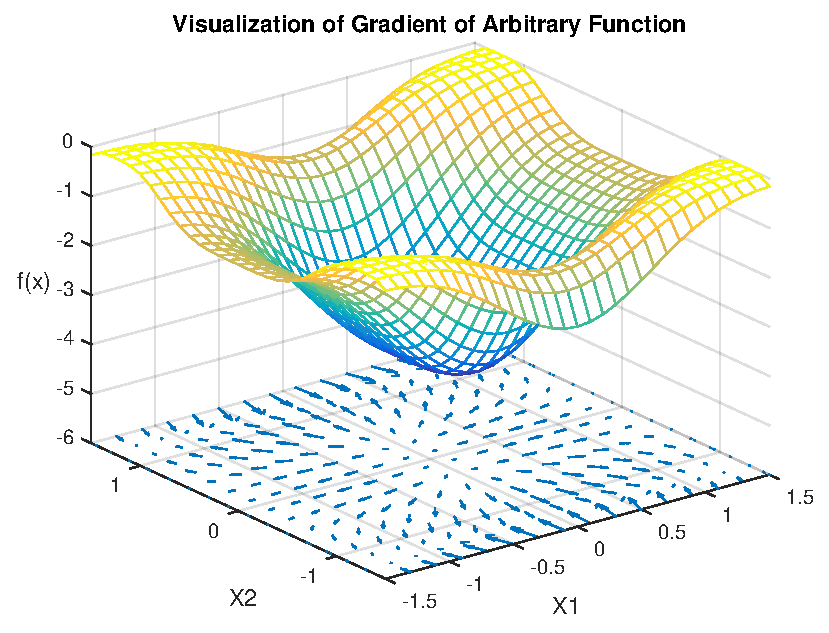
\includegraphics[width=.8\textwidth]{figures/visualizationOfGradient}
	\caption{Visualization of gradient of an arbitrary function.}
	\label{visualizationOfGradient}
\end{figure}

One way of implementation is to set a step-size which decides how far in the \si{-\vec{g}} direction to go. The step-size can then be scaled in each iteration to avoid taking too large steps as shown in \figref{SteepestDescendLargeStep} and \ref{SteepestDescendSmallStep}, where \si{x^*} is the value of \si{x} which minimizes \si{f(x)}, \si{x_0} is the starting point at which \si{-g} is computed and \si{x} is the point reached after the step.
%
\begin{minipage}{\linewidth}
	\begin{minipage}{0.45\linewidth}
		\begin{figure}[H]
			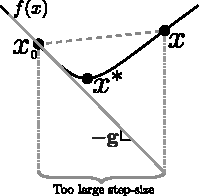
\includegraphics[scale=1.4]{figures/gradientDescendLargeStep2}
			\centering
			\captionsetup{justification=centering}
			\captionof{figure}{A too large step will cause the algorithm to step over the valley, resulting in a larger value of f(x) in the \si{-\vec{g}} direction.}
			\label{SteepestDescendLargeStep}
		\end{figure}
	\end{minipage}
	\hspace{0.03\linewidth}
	\begin{minipage}{0.45\linewidth}
		\begin{figure}[H]
			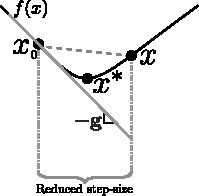
\includegraphics[scale=1.44]{figures/gradientDescendReducedStep2}
			\centering
			\captionsetup{justification=centering}
			\captionof{figure}{By going back and choosing a smaller step, a smaller value for f(x) is obtained.}
			\label{SteepestDescendSmallStep}
		\end{figure}
	\end{minipage}
\end{minipage}

The steepest descend method does find a minimum. However, it converges to it rather slowly. An implementation where it is possible to directly retrieve the gradient of the function which is to be minimized, \si{f(\vec{x})}, is shown in \figref{steepestDescendEx}.

\begin{minipage}{\linewidth}
	\begin{minipage}{0.45\linewidth}
		\begin{figure}[H]
			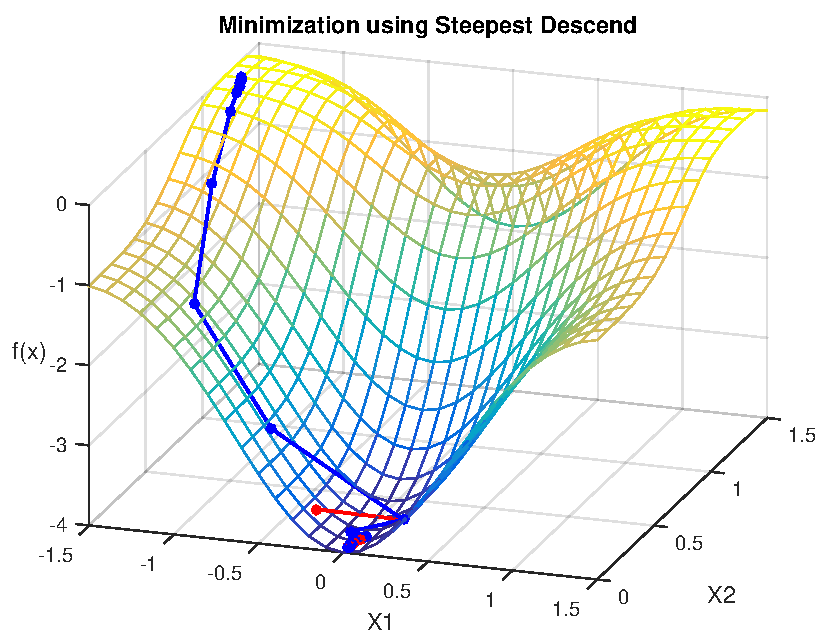
\includegraphics[scale=.6]{figures/steepestDescendEx}
			\centering
			\captionsetup{justification=centering}
			\captionof{figure}{An example of a direct implementation of the steepest descend method. It steps over the valley and the step size is reduced in the red iteration.}
			\label{steepestDescendEx}
		\end{figure}
	\end{minipage}
	\hspace{0.03\linewidth}
	\begin{minipage}{0.45\linewidth}
		\begin{figure}[H]
			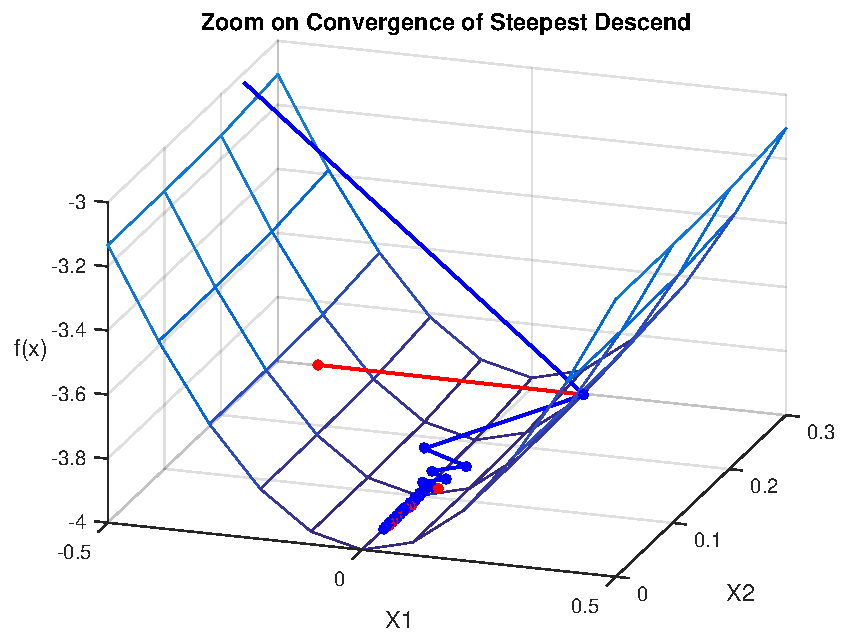
\includegraphics[scale=.6]{figures/steepestDesendExZoom}
			\centering
			\captionsetup{justification=centering}
			\captionof{figure}{From the zoom on the convergence, it is seen that many iterations (here 100) are needed using this method.\vspace{12pt}}
			\label{steepestDesendExZoom}
		\end{figure}
	\end{minipage}
\end{minipage}

%From the zoom on \figref{steepestDesendExZoom} the convergence toward %the minimum is clear, however it is also clear that many iterations are %needed to get there.

\subsection{Newton's Method}
Another approach is called Newton's Method, which is also rooted in the Taylor approximation. However, this method also uses the second order term of the approximation.
%
\begin{flalign}
  f(\vec{x}+\vec{\delta}) &\approx f(\vec{x}) + \vec{g}^T \vec{\delta} + \frac{1}{2} \vec{\delta}^T \vec{H}\vec{\delta} &
\label{taylorApproximation2ndOrder}
\end{flalign}

In this case the derivative of the approximation is set to 0, and the following is obtained.
%
\begin{flalign}
  \frac{\partial}{\partial \vec{\delta}} \ f(\vec{x}+\vec{\delta}) &\approx \vec{g} + \frac{1}{2}\ \frac{\partial}{\partial \vec{\delta}}\ \vec{H}\vec{\delta}^2 &\\
  \frac{\partial}{\partial \vec{\delta}} \ f(\vec{x}+\vec{\delta}) &\approx \vec{g} + \vec{H}\vec{\delta} = 0 &
\label{2stOrderTaylorApproximationParThetaEqZero}
\end{flalign}

Using this to find an expression for the difference in \si{\vec{x}}, \si{\vec{\delta}}, yields the following.
%
\begin{flalign}
  0 &= \vec{g} + \vec{H}\vec{\delta}  &\\
  \vec{\delta} &= -\vec{H}^{-1}\vec{g} &
\label{NewtonsMethod}
\end{flalign}

This expression can then be used to choose the value of \si{\vec{\delta}} such that the approximation of \si{f(\vec{x})} is minimized. An implementation where it is possible to directly retrieve the gradient and a Hessian of the function which is to be minimized, \si{f(\vec{x})}, is shown in \figref{NewtonsMethodEx}. 
%
\begin{figure}[H] 
	\centering
	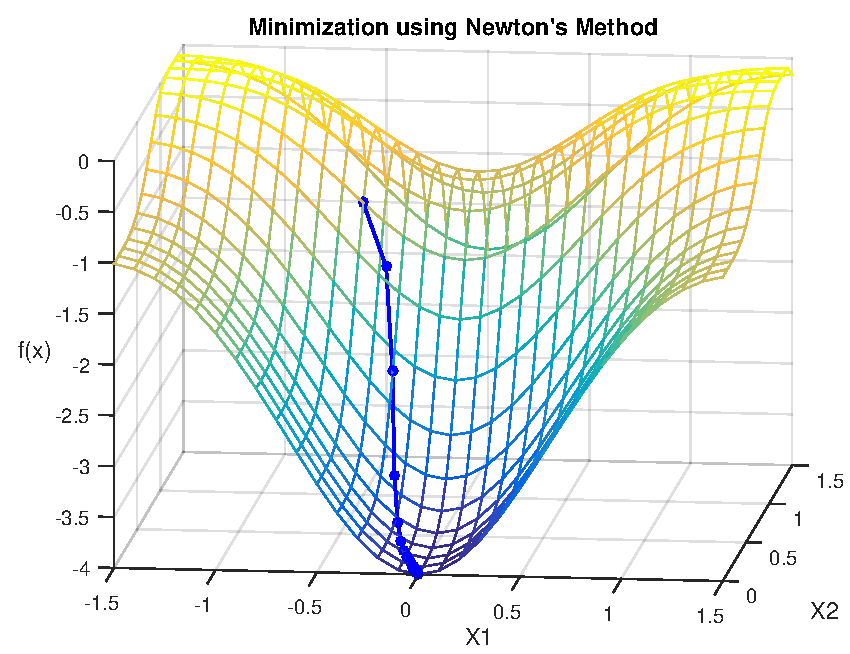
\includegraphics[width=.7\textwidth]{figures/NewtonsMethodEx}
	\caption{Example of a direct implementation of Newton's method for optimization.}
	\label{NewtonsMethodEx}
\end{figure}

If compared to the steepest descend method in \figref{steepestDescendEx} and \ref{steepestDesendExZoom}, where 100 iterations were used, it is clear how Newton's method converges much faster, in 30 iterations, to the minimum of \si{f(\vec{x})}. 

\subsection{Implementation of Newton's Method}
When implementing Newton's Method both the gradient and the Hessian of the performance function \eqref{performanceFunction} are needed.
%
\begin{flalign}
	\frac{\partial  }{\partial \vec{\theta}} P(\vec{\theta}) &= \vec{G}(\vec{\theta}) = \frac{\partial}{\partial \vec{\theta}} \left( \frac{1}{2N}\sum_{k = 1}^{N} \left(\vec{y}(kT) - \vec{y_m}(kT, \vec{\theta})\right)^2 \right) &
\end{flalign}
\begin{flalign}
  \eq{\vec{G}(\vec{\theta})} {- \frac{1}{N}\sum_{k = 1}^{N} \left((\vec{y}(kT) - \vec{y_m}(kT, \vec{\theta})) \ \frac{\partial  }{\partial \vec{\theta}} \ \vec{y_m}(kT, \vec{\theta}) \right) } &
\label{gradientOfPerformanceFunction}
\end{flalign}
%\begin{flalign}
%	\frac{\partial \vec{P}(\vec{\theta}) }{\partial \vec{\theta}} &= G(\vec{\theta}) = \frac{\partial}{\partial \vec{\theta}} \left( \frac{1}{2N}\sum_{k = 1}^{N} \left(\vec{y}(kT) - \vec{y_m}(kT, \vec{\theta})\right)^2 \right) &\\
%  \eq{\vec{G}(\vec{\theta})} {- \frac{1}{N}\sum_{k = 1}^{N} \left((\vec{y}(kT) - \vec{y_m}(kT, \vec{\theta})) \ \frac{\partial  \vec{y_m}(kT, \vec{\theta})}{\partial \vec{\theta}} \right) } &
%\label{gradientOfPerformanceFunction}
%\end{flalign}

Since the Matlab implementation uses a Simulink model the problematic part of \eqref{gradientOfPerformanceFunction} is the derivative of the model with respect to the model parameters, \si{\frac{\partial  }{\partial \vec{\theta}}\ \vec{y_m}(kT, \vec{\theta})}. To solve this problem a numerical differentiation of the model is applied as shown in \autoref{AlgorithmForNummericalDiff}.

\begin{lstlisting}[ language = Matlab,
                    caption  = {Algorithm for numerical differentiation of the simulated model},
                    label    = AlgorithmForNummericalDiff ]

  %small deviation from parameters, J_f and B_f, is set
  p = 0.001;
  
  %calculating the deviation
  deltaJ_f = p*J_f; deltaB_f = p*B_f;
  
  %saving the old parameters:
  J_f_old = J_f; B_f_old = B_f;
  
  %setting deviating parameters ready for simulation
  J_f = deltaJ_f;
  
  %running the simulation again, now with deviation in J_f
  sim('CubliParameterEstimation.slx');
  
  %storring the result of the simulation
  deltaYmJf = simOut;
  
  %setting deviating parameters ready for simulation
  B_f = deltaB_f; J_f = J_f_old; %<--restoring J_f
  
  %running the simulation again, now with deviation in B_f
  sim('CubliParameterEstimation.slx');
  
  %storring the result of the simulation
  deltaYmBf = simOut;
  
  %restoring the parameters to their original value
  B_f = B_f_old;
  
  %calculating the derivatives of the model
  YmDiffBf = ( deltaYmBf - Ym )/ p;
  YmDiffJf = ( deltaYmJf - Ym )/ p;
\end{lstlisting}

Now that the model partial derivatives are found, all parts of the gradient, as represented in \eqref{gradientOfPerformanceFunction}, are known. The Hessian is also needed and can be represented as,
%
\begin{flalign}
	\vec{H}(\vec{\theta}) &= \frac{\partial^2 }{\partial \vec{\theta}^2}\  P(\vec{\theta}) = \frac{\partial }{\partial \vec{\theta}} \ \vec{G}(\vec{\theta}) &
\end{flalign}
%
which leads to the following:
\begin{flalign}
	\vec{H}(\vec{\theta}) &= \frac{1}{N}\sum_{k = 1}^{N} \left(     \frac{\partial  }{\partial \vec{\theta}} \ \vec{y_m}(kT, \vec{\theta}) \left(\frac{\partial }{\partial \vec{\theta}} \ \vec{y_m}(kT, \vec{\theta}) \right)^T  	  - \left(\frac{\partial^2  }{\partial \vec{\theta}^2} \ \vec{y_m}(kT, \vec{\theta}) \right) (\vec{y}(kT) - \vec{y_m}(kT, \vec{\theta}))  \right) &
\label{hessianOfPerformanceFunction}
\end{flalign}
%\begin{flalign}
%	\vec{H}(\vec{\theta}) &= \frac{1}{N}\sum_{k = 1}^{N} \left(   \left\Vert \frac{\partial  \vec{y_m}(kT, \vec{\theta})}{\partial \vec{\theta}} \right\Vert_2^2  	  - \left(\frac{\partial^2 \vec{y_m}(kT, \vec{\theta}) }{\partial^2 \vec{\theta}^2}\right) (\vec{y}(kT) - \vec{y_m}(kT, \vec{\theta}))  \right) &
%\label{hessianOfPerformanceFunction}
%\end{flalign}
%\begin{flalign}
%	\vec{H}(\vec{\theta}) &= \frac{1}{N}\sum_{k = 1}^{N} \left(   \frac{\partial  \vec{y_m}(kT, \vec{\theta})}{\partial \vec{\theta}} \left(\frac{\partial \vec{y_m}(kT, \vec{\theta})}{\partial \vec{\theta}} \right)^T  	  - \left(\frac{\partial^2 \vec{y_m}(kT, \vec{\theta}) }{\partial^2 \vec{\theta}^2}\right) (\vec{y}(kT) - \vec{y_m}(kT, \vec{\theta}))  \right) &
%\label{hessianOfPerformanceFunction}
%\end{flalign}
%
To avoid the second derivative of the performance function in \eqref{hessianOfPerformanceFunction}, the Hessian can be approximated simply by removing this last term.
\begin{flalign}
	\vec{\widetilde{H}}(\vec{\theta}) &\triangleq \frac{1}{N}\sum_{k = 1}^{N} \frac{\partial  }{\partial \vec{\theta}} \ \vec{y_m}(kT, \vec{\theta}) \left(\frac{\partial }{\partial \vec{\theta}} \ \vec{y_m}(kT, \vec{\theta}) \right)^T &
\label{hessianApproxOfPerformanceFunction}
\end{flalign}
%\begin{flalign}
%	\vec{\widetilde{H}}(\vec{\theta}) &\triangleq \frac{1}{N}\sum_{k = 1}^{N} \ \left\Vert  \frac{\partial  \vec{y_m}(kT, \vec{\theta})}{\partial \vec{\theta}} \right\Vert_2^2 &
%\label{hessianApproxOfPerformanceFunction}
%\end{flalign}
%\begin{flalign}
%	\vec{\widetilde{H}}(\vec{\theta}) &\triangleq \frac{1}{N}\sum_{k = 1}^{N} \left(   \frac{\partial  \vec{y_m}(kT, \vec{\theta})}{\partial \vec{\theta}} \left(\frac{\partial \vec{y_m}(kT, \vec{\theta})}{\partial \vec{\theta}} \right)^T \right) &
%\label{hessianApproxOfPerformanceFunction}
%\end{flalign}
%
This approximation assumes that the model is only linearly dependent on the parameters, \si{\vec{\theta}}. As the error term, \si{(\vec{y}(kT) - \vec{y_m}(kT, \vec{\theta}))}, approaches zero the approximation becomes increasingly accurate.

Running the implementation of Newton's method approximates the model parameters to \si{J_F = } and \si{B_F = }, while giving a normed root mean square error of \si{31,71 \%} as seen on \figref{ParameterEstimationNewtonCubli}. %The normed RMS error is a way to determine the goodness of the fit.

\begin{figure}[H] 
	\centering
	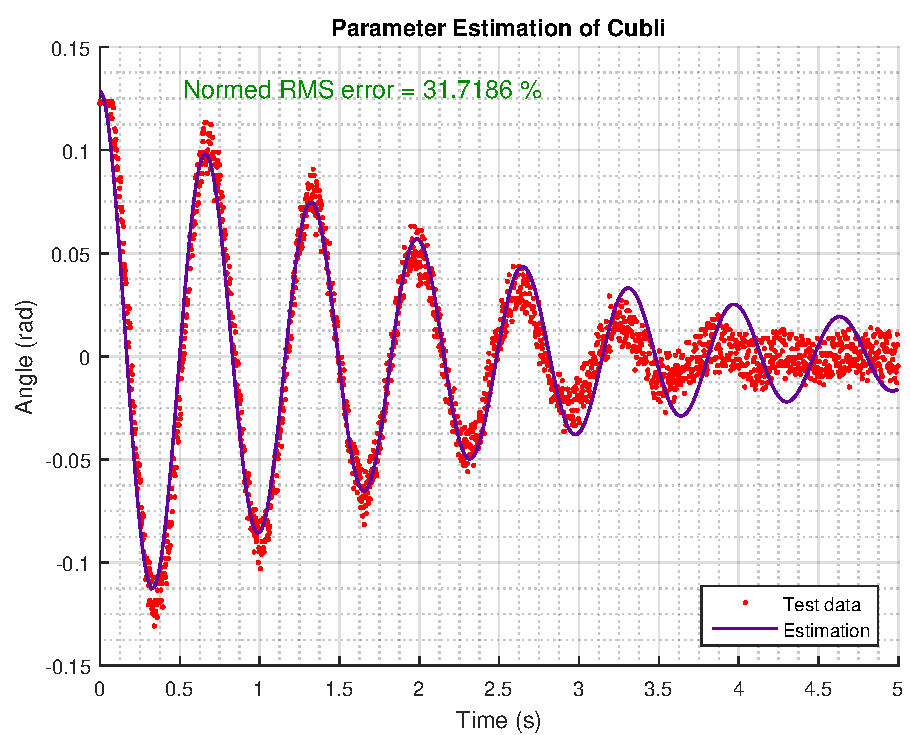
\includegraphics[width=.8\textwidth]{figures/ParameterEstimationNewtonCubli}
	\caption{The result of implementation of Newton's method}
	\label{ParameterEstimationNewtonCubli}
\end{figure}

\subsection{SensTool}
A lot of the background for the implementation above comes from documentation on a Matlab toolbox called SensTool \fxnote{Reference Senstool guide}. The optimization method is implemented in it and it also includes an extra feature based on parameter sensitivity and frequency domain. For a better accuracy on the estimation it is a good decision to use this tool as the final approach to the parameters of the Cubli model.

The same data, Simulink model and initial parameters as the previous case are given to this toolbox and the result of the fit can be seen in \figref{SenseToolParameterEstimation}. 
%
\begin{figure}[H]
	\centering
	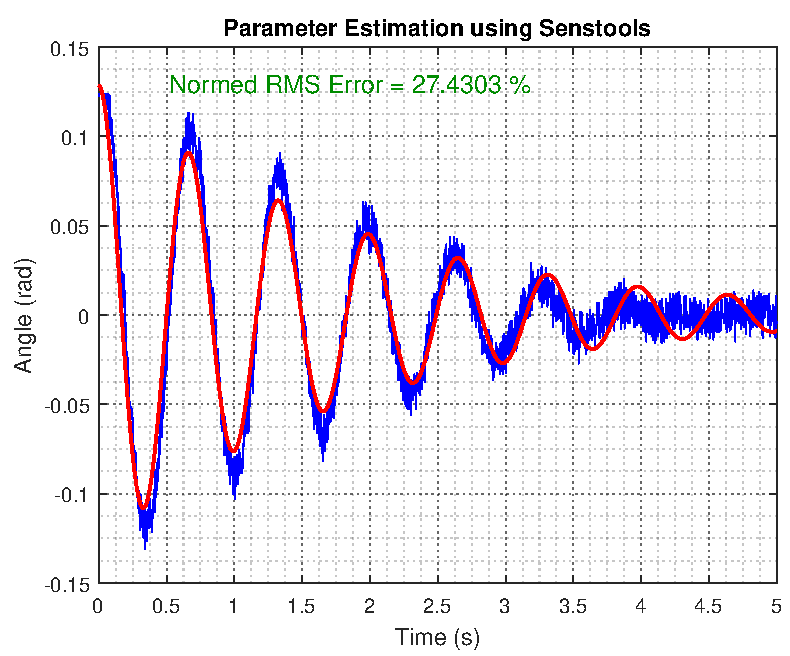
\includegraphics[scale=0.6]{figures/SenseToolParameterEstimation}
	\caption{Data from the test (red) and final fit with the new parameters (blue)}
	\label{SenseToolParameterEstimation}
\end{figure}
%

The final estimated parameters are \si{J_F=4,8 \cdot 10^{-3}\ kg \cdot m^2\ and\ B_F=7,7 \cdot 10^{-3}\ m \cdot s \cdot rad^{-1}}. The normed RMS error is \si{27,4\ \%} compared to the \si{31,7\ \%} shown in \figref{ParameterEstimationNewtonCubli}. The \si{4,3\ \%} error reduction is likely due to additional algorithms.

\section{Final Parameters}
The final parameters of the system can be seen in \ref{ParametersSystem}
\begin{table}[H]
	\begin{tabular}{|l|l|p{3cm}|}
		\hline %-----------------------------------------------------------------------------------
		\textbf{Parameter} &\textbf{Value} &\textbf{Units}\\
		\hline %-----------------------------------------------------------------------------------
		\si{m_w}         & \si{0,222}       &kg\\
		\hline
		%-----------------------------------------------------------------------------------
		\si{l_w}         & \si{0,096}       &m\\
		\hline %-----------------------------------------------------------------------------------
		\si{J_w}            & \si{0,601 \cdot 10^{-3}}	&\si{kg \cdot m^2}\\
		\hline  
		%-----------------------------------------------------------------------------------
		\si{B_w}         & \si{17,03 \cdot 10^{-6}}       &N \si{\cdot m \cdot s \cdot rad^{-1}}\\
		\hline
		%-----------------------------------------------------------------------------------
		\si{m_F}         & \si{0,548}       &kg\\
		\hline
		%-----------------------------------------------------------------------------------
		\si{l_F}         & \si{0,08498}       &m\\
		\hline %-----------------------------------------------------------------------------------
		\si{J_F}            & \si{4,8 \cdot 10^{-3}}	&\si{kg \cdot m^2}\\
		\hline %-----------------------------------------------------------------------------------
		\si{B_F}         & \si{7,7 \cdot 10^{-3}}       &N \si{\cdot m \cdot s \cdot rad^{-1}}\\
		\hline
	\end{tabular}
	\caption{Parameters of the whole system}
	\label{ParametersSystem}
\end{table}